\documentclass{beamer}

\usepackage[utf8]{inputenc}
\usepackage[T1]{fontenc}

\title{A beamer template for the OR Group}
\date{\today}
\author[Alberto]{Alberto Santini\\\texttt{a.santini@unibo.it}}

\usetheme{orbo}

\begin{document}

\begin{frame}
  \titlepage
\end{frame}

\begin{frame}{Plan}
  \tableofcontents
\end{frame}

\section{A theorem in $MA(\kappa)$}

\begin{frame} 
  \frametitle{A theorem in $MA(\kappa)$} 
  \framesubtitle{A classical theorem related to Martin's Axiom} 
  
  \begin{theorem}
    Let $\kappa$ be an infinite cardinal and assume $MA(\kappa)$. Given $A,B \in \mathcal{P}(\omega)$ with $|A|,|B| \leq \kappa$, if
    \begin{equation*}
      \forall b \in B, \; \forall F \in [A]^{<\omega} \quad \left| b \cap \bigcup F \right| = \omega
    \end{equation*}
    Then $\exists c \subset \omega$ such that $|c \cap a| < \omega$ for all $a \in A$ while $|c \cap b| = \omega$ for all $b \in B$.
  \end{theorem}
  
\end{frame}

\begin{frame}{A theorem in $MA(\kappa)$}
  \begin{enumerate} 
    \item<1-> The proof proceeds by first proving that the set $X^b_n = \{ (s, F) \in \mathbb{P}_A \ | \ s \cap b \not\subseteq n \}$ is dense for all $b \in B$ and $n \in \omega$
    \item<2-> By $MA(\kappa)$ we can then produce a filter $G$ on $\mathbb{P}_A$ that intersects all the sets $X^b_n$
    \item<3-> The theorem follows, with $c = \bigcup_{(s,F) \in G} s$
  \end{enumerate}
\end{frame}

\section{Pro Publio Quinctio}

\begin{frame}{Pro Publio Quinctio}
  Opinor, tuum testimonium, quod in aliena re leve esset, id in tua, quoniam contra te est, gravissimum debet esse. Emisti bona Sex. Alfeni L. Sulla dictatore vendente; socium tibi in his bonis edidisti Quinctium.
  \vspace{1em}
  \begin{center}
    \textcolor{unibored}{Plura non dico.}
  \end{center}
\end{frame}

\begin{frame}{Pro Publio Quinctio}
  \begin{itemize}
    \item<1-> Miserum est exturbari fortunis omnibus, miserius est \textcolor{uniboblue}{iniuria};
    \item<2-> Acerbum est ab aliquo circumveniri, acerbius a propinquo;
    \item<3-> Calamitosum est bonis everti calamitosius cum dedecore;
    \item<4-> Funestum est a forti atque \textcolor{unibored}{honesto viro iugulari}, funestius ab eo cuius vox in praeconio quaestu prostitit;
    \item<5-> Indignum est a pari vinci aut superiore, indignius ab inferiore atque humiliore;
    \item<6-> Luctuosum est tradi alteri cum bonis, luctuosius inimico;
    \item<7-> Horribile est causam capitis dicere, horribilius priore loco dicere.
  \end{itemize}
\end{frame}

\section{Results}

\begin{frame}{Results}
  \begin{center}\resizebox{!}{0.5\paperheight}{
    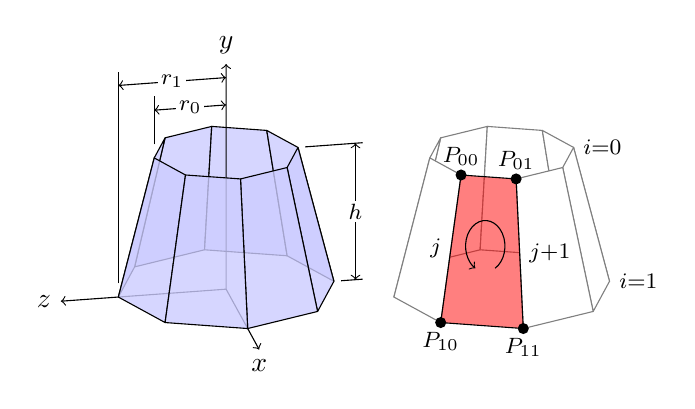
\begin{tikzpicture}[join=round]
        \tikzstyle{conefill} = [fill=blue!20,fill opacity=0.8]
        \tikzstyle{ann} = [fill=white,font=\footnotesize,inner sep=1pt]
        \tikzstyle{ghostfill} = [fill=white]
             \tikzstyle{ghostdraw} = [draw=black!50]
        \filldraw[conefill](-.775,1.922)--(-1.162,.283)--(-.274,.5)
                            --(-.183,2.067)--cycle;
        \filldraw[conefill](-.183,2.067)--(-.274,.5)--(.775,.424)
                            --(.516,2.016)--cycle;
        \filldraw[conefill](.516,2.016)--(.775,.424)--(1.369,.1)
                            --(.913,1.8)--cycle;
        \filldraw[conefill](-.913,1.667)--(-1.369,-.1)--(-1.162,.283)
                            --(-.775,1.922)--cycle;
        \draw(1.461,.107)--(1.734,.127);
        \draw[arrows=<->](1.643,1.853)--(1.643,.12);
        \filldraw[conefill](.913,1.8)--(1.369,.1)--(1.162,-.283)
                            --(.775,1.545)--cycle;
        \draw[arrows=->,line width=.4pt](.274,-.5)--(0,0)--(0,2.86);
        \draw[arrows=-,line width=.4pt](0,0)--(-1.369,-.1);
        \draw[arrows=->,line width=.4pt](-1.369,-.1)--(-2.1,-.153);
        \filldraw[conefill](-.516,1.45)--(-.775,-.424)--(-1.369,-.1)
                            --(-.913,1.667)--cycle;
        \draw(-1.369,.073)--(-1.369,2.76);
        \draw(1.004,1.807)--(1.734,1.86);
        \filldraw[conefill](.775,1.545)--(1.162,-.283)--(.274,-.5)
                            --(.183,1.4)--cycle;
        \draw[arrows=<->](0,2.34)--(-.913,2.273);
        \draw(-.913,1.84)--(-.913,2.447);
        \draw[arrows=<->](0,2.687)--(-1.369,2.587);
        \filldraw[conefill](.183,1.4)--(.274,-.5)--(-.775,-.424)
                            --(-.516,1.45)--cycle;
        \draw[arrows=<-,line width=.4pt](.42,-.767)--(.274,-.5);
        \node[ann] at (-.456,2.307) {$r_0$};
        \node[ann] at (-.685,2.637) {$r_1$};
        \node[ann] at (1.643,.987) {$h$};
        \path (.42,-.767) node[below] {$x$}
            (0,2.86) node[above] {$y$}
            (-2.1,-.153) node[left] {$z$};
        % Second version of the cone
        \begin{scope}[xshift=3.5cm]
        \filldraw[ghostdraw,ghostfill](-.775,1.922)--(-1.162,.283)--(-.274,.5)
                                       --(-.183,2.067)--cycle;
        \filldraw[ghostdraw,ghostfill](-.183,2.067)--(-.274,.5)--(.775,.424) 
                                       --(.516,2.016)--cycle;
        \filldraw[ghostdraw,ghostfill](.516,2.016)--(.775,.424)--(1.369,.1)
                                       --(.913,1.8)--cycle;
        \filldraw[ghostdraw,ghostfill](-.913,1.667)--(-1.369,-.1)--(-1.162,.283)
                                       --(-.775,1.922)--cycle;
        \filldraw[ghostdraw,ghostfill](.913,1.8)--(1.369,.1)--(1.162,-.283)
                                       --(.775,1.545)--cycle;
        \filldraw[ghostdraw,ghostfill](-.516,1.45)--(-.775,-.424)--(-1.369,-.1)
                                       --(-.913,1.667)--cycle;
        \filldraw[ghostdraw,ghostfill](.775,1.545)--(1.162,-.283)--(.274,-.5)
                                       --(.183,1.4)--cycle;
        \filldraw[fill=red,fill opacity=0.5](-.516,1.45)--(-.775,-.424)--(.274,-.5)
                                             --(.183,1.4)--cycle;
        \fill(-.775,-.424) circle (2pt);
        \fill(.274,-.5) circle (2pt);
        \fill(-.516,1.45) circle (2pt);
        \fill(.183,1.4) circle (2pt);
        \path[font=\footnotesize]
                (.913,1.8) node[right] {$i\hbox{$=$}0$}
                (1.369,.1) node[right] {$i\hbox{$=$}1$};
        \path[font=\footnotesize]
                (-.645,.513) node[left] {$j$}
                (.228,.45) node[right] {$j\hbox{$+$}1$};
        \draw (-.209,.482)+(-60:.25) [yscale=1.3,->] arc(-60:240:.25);
        \fill[black,font=\footnotesize]
                        (-.516,1.45) node [above] {$P_{00}$}
                        (-.775,-.424) node [below] {$P_{10}$}
                        (.183,1.4) node [above] {$P_{01}$}
                        (.274,-.5) node [below] {$P_{11}$};
        \end{scope}
    \end{tikzpicture}
  }\end{center}
\end{frame}

\end{document}